\part{Comparison} \label{part:Comparison and implementation}

\chapter{comparisons and implementations}

\section{t-SNE}
There are 4 most important parameters for t-SNE, the basic ideas of each parameters are: 

\begin{enumerate}[1)]
\item $perplexity$: number of nearest neighbors for each point
\item $n\_iter$: maximum number of iterations for optimization
\item $early\_exaggeration$: the tightness inside clusters and the distance inbetween
\item $min\_grad\_norm$: the threshold for stopping the optimization 
\end{enumerate}\\

\noindent In order to draw the conclusions in a convincing way, This work examines the three algorithms' quality on several real-world data sets with different level of instances and dimensions, base on the neighborhood-based DR performance criteria discussed above. there are six public databases: Iris, Wine, Breast Cancer Wisconsin Diagnostic (BCW), Optical Recognition of Handwritten Digits test set (Digits), the B. Frey’s images (B.Freys) and Labeled Faces in the Wild face recognition(LFW).\\

\begin{center}
\begin{tabular}{|c|c|c|}% 通过添加 | 来表示是否需要绘制竖线
\hline  % 在表格最上方绘制横线
Datasets & Number of instances & Number of dimensions\\
\hline  %在第一行和第二行之间绘制横线
Iris & 150 & 4\\
\hline  %在第一行和第二行之间绘制横线
Wine & 178 & 13\\
\hline  %在第一行和第二行之间绘制横线
BCW & 569 & 30\\
\hline  %在第一行和第二行之间绘制横线
digit & 1797 & 64\\
\hline  %在第一行和第二行之间绘制横线
B.Freys & 1965 & 560\\
\hline  %在第一行和第二行之间绘制横线
LFW & 13233 & 5749\\
\hline % 在表格最下方绘制横线
\end{tabular}\\
\end{center}
\\

\noindent When we are analyzing the result, we should consider that the high-dimensional sphere was modeled by probability graph, the t-SNE algorithm adapts its "distance" concept to changes in regional density in the data set. As a result, it naturally expands dense clusters and shrinks sparse clusters, making the clusters roughly uniform in size. It also makes it difficult to see the relative size of clusters in the t-SNE graph, and the distance between clusters in low dimensions does not represent the distance between clusters in high dimensions.

\subsection{$perplexity$}

\noindent The first adjustable parameter of t-SNE represent the number of neighbors each point t-SNE considers. It explains how to maintain a balance between the local and global aspects of the data. The perplexity value has a complex effect on the generated pictures, but the performance of SNE is quite reliable for changes in complexity, and the typical value of perplexity is between 5 and 50\cite{ref9}. Also, since the perplexity means the number of the neighbors, it should not be higher than the number of data points.\\

\noindent We can try different potential perplexity values in datasets with different instances. At the same time, since the algorithm using stochastic method, the parameter $random\_state$ is set to 1. This parameter determines the random number generator so that it pass an int mark for reproducible results across multiple function calls. After examining it on the first dataset Iris, we get the figures below:

\begin{figure}[H]
\centering  %图片全局居中
% \subfigure[name1]
{
\label{Fig.sub.1}
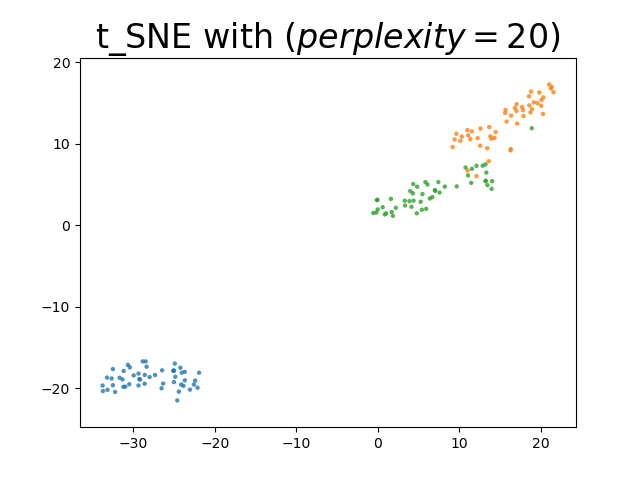
\includegraphics[width=7cm,height=3.5cm\textwidth]{images/image_comparison_tsne_perp20.png}}
% \subfigure[name2]
{
\label{Fig.sub.2}
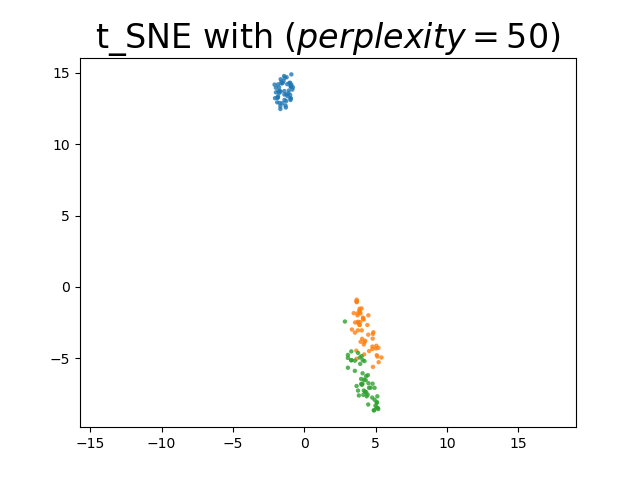
\includegraphics[width=7cm,height=3.5cm\textwidth]{images/image_comparison_tsne_perp50.png}}
% \caption{Main name}
% \label{Fig.main}
\end{figure}

\begin{figure}[H]
\centering  %图片全局居中
% \subfigure[name1]
{
\label{Fig.sub.1}
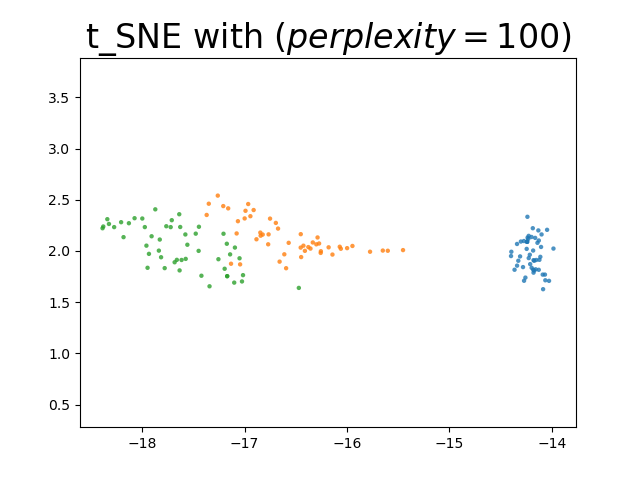
\includegraphics[width=7cm,height=3.5cm\textwidth]{images/image_comparison_tsne_perp100.png}}
% \subfigure[name2]
{
\label{Fig.sub.2}
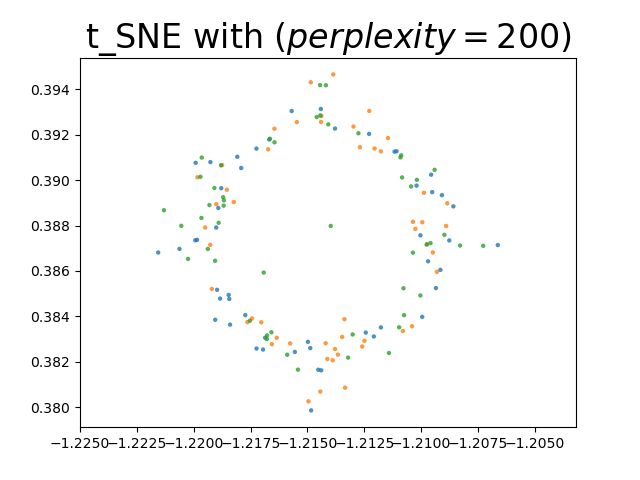
\includegraphics[width=7cm,height=3.5cm\textwidth]{images/image_comparison_tsne_perp200.png}}
\caption{LD result for t-SNE with different perplexity}
% \label{Fig.main}
\end{figure}


\noindent In the figure, we can see that when the value is in the range of 5-50, clusters are well distinguished. Considering that the number of instances of the dataset is only 150, when the value is 100, the clusters begin to merge. When the perplexity = 200, it is difficult to distinguish different clusters. In order for the algorithm to work properly, the perplexity should actually be less than the number of points. Considering the experimental results and the strategy of the search about the optimal number of neighbor from K nearest neighbour algorithm\cite{ref12}, we can simply set perplexity to $n^{0.5}$, where n stand for number of instances. \\

\noindent At the same time, the $AUC$ value for the result with these parameters are 0.731, 0.658, 0.654, -0.004 separately. These $AUC$ values verifies the previous observations. As for the last one, it has a big difference between others and also the only minus result. With the definition of the $R_{NX}$ curve $R_{NX} (K) = ((N − 1)Q_{NX} (K) − K) /(N − 1 − K)$, this is because the K is higher than N in the formula. Numerator is relative small and denominator is a negative number, we then have a minus result.


\subsection{$n\_iter$}

\noindent $n\_iter$ is the maximum number of iterations for the algorithm. The graph observed above are all generated with 1000 iteration which is the default value of $n\_iter$. In principle, the higher $n\_iter$ gives the better result. However, it may be very time consuming when it comes to big dataset. In contrast, if $n\_iter$ is too small, the algorithm does not have enough iteration to generate the convincing clusters in LD. The most important thing is to reach a stable configuration. The figure shows how the result changes with $n\_iter$ grows in the same Iris dataset as above:

\begin{figure}[H]
\centering  %图片全局居中
% \subfigure[name1]
{
\label{Fig.sub.1}
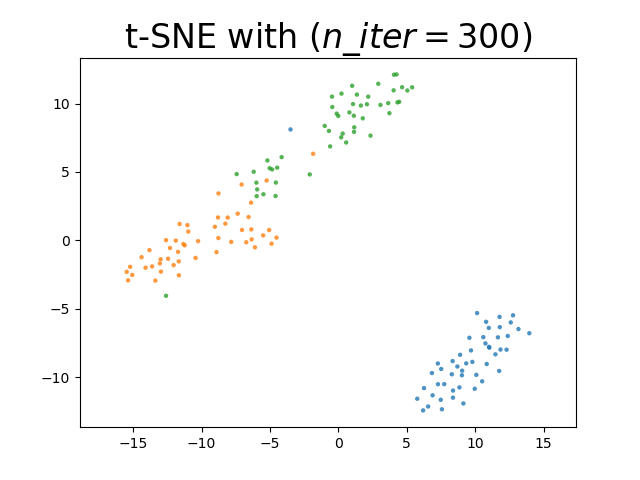
\includegraphics[width=7cm,height=3.5cm\textwidth]{images/t-sne/t-sne_n_iter_300.png}}
% \subfigure[name2]
{
\label{Fig.sub.2}
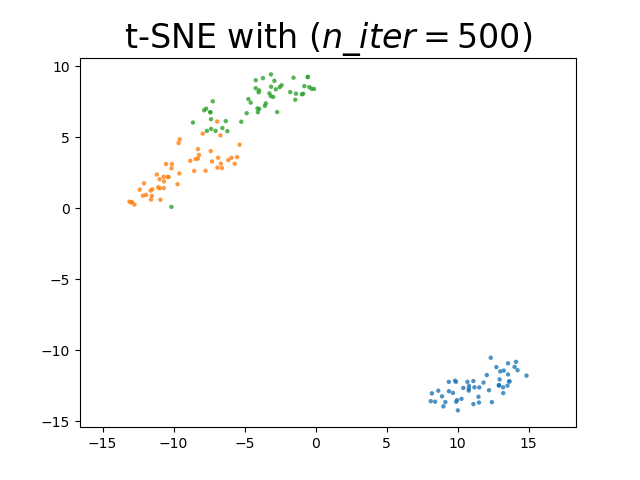
\includegraphics[width=7cm,height=3.5cm\textwidth]{images/t-sne/t-sne_n_iter_500.png}}
\caption{LD result for t-SNE with n\_iter 300 and 500}
% \label{Fig.main}
\end{figure}

\begin{figure}[H]
\centering  %图片全局居中
% \subfigure[name1]
{
\label{Fig.sub.1}
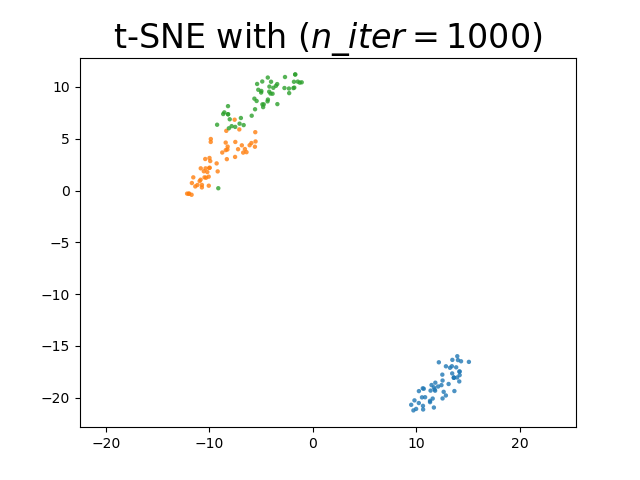
\includegraphics[width=7cm,height=3.5cm\textwidth]{images/t-sne/t-sne_n_iter_1000.png}}
% \subfigure[name2]
{
\label{Fig.sub.2}
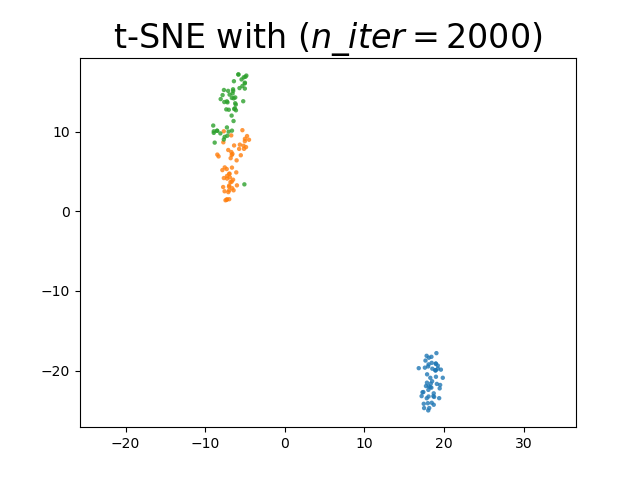
\includegraphics[width=7cm,height=3.5cm\textwidth]{images/t-sne/t-sne_n_iter_2000.png}}
\caption{LD result for t-SNE with n\_iter 1000 and 2000}
% \label{Fig.main}
\end{figure}

\noindent From the figure, we can easily observe that the more iterations, the more well identified for clusters. These four $n\_iter$ generate $AUC$ values for 0.622, 0.654, 0.670, 0.692 separately, which verified the previous conclusion. 

% 上图显示了在困惑度30下的五个不同的运行。前四个在稳定之前已停止。经过10、20、60和120步后,您可以看到带有簇的一维甚至点状图像的布局。如果您看到t-SNE图上有奇怪的“挤压”形状,则该过程可能停止得太早。经过六个不同维度数据集的测试,改参数没有固定的数值可以产生稳定结果。不同的数据集可能需要不同数量的迭代才能收敛。

% 之后还有perp与n_iter之间的heatmap,解释一波

\subsection{$early\_exaggeration$}

$ early\ _exaggeration $ controls the closeness of clusters in high-dimensional space and the distance between them in low-dimensional space. For larger values, the space between natural clusters will be larger in the embedded space. As analyzed before, the distance between the low-dimensional space and the tightness of clustering have limited influence on the result, so this parameter has a small influence on the $AUC$ result. But if the cost function is increased during the initial optimization process, the early exaggeration factor may be too high.

\subsection{$min\_grad\_norm$}

This parameter is the threshold of gradient norm to determine when the optimization will be stopped.